

\tikzset{every picture/.style={line width=0.75pt}} %set default line width to 0.75pt        

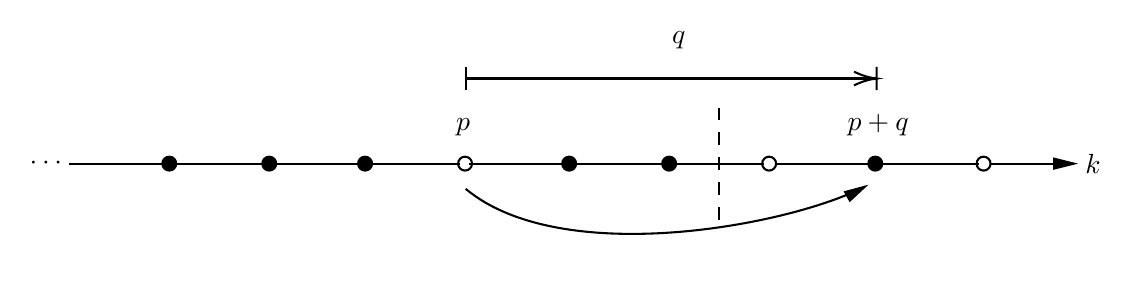
\begin{tikzpicture}[x=0.75pt,y=0.75pt,yscale=-1,xscale=1]
%uncomment if require: \path (0,300); %set diagram left start at 0, and has height of 300

%Straight Lines [id:da4100443293723468] 
\draw    (120,122) -- (168.17,122) ;
\draw [shift={(168.17,122)}, rotate = 0] [color={rgb, 255:red, 0; green, 0; blue, 0 }  ][fill={rgb, 255:red, 0; green, 0; blue, 0 }  ][line width=0.75]      (0, 0) circle [x radius= 3.35, y radius= 3.35]   ;
%Straight Lines [id:da8268118303886198] 
\draw    (168.17,122) -- (216.33,122) ;
\draw [shift={(216.33,122)}, rotate = 0] [color={rgb, 255:red, 0; green, 0; blue, 0 }  ][fill={rgb, 255:red, 0; green, 0; blue, 0 }  ][line width=0.75]      (0, 0) circle [x radius= 3.35, y radius= 3.35]   ;
%Straight Lines [id:da43623564624457467] 
\draw    (214.33,122) -- (262.5,122) ;
\draw [shift={(262.5,122)}, rotate = 360] [color={rgb, 255:red, 0; green, 0; blue, 0 }  ][fill={rgb, 255:red, 0; green, 0; blue, 0 }  ][line width=0.75]      (0, 0) circle [x radius= 3.35, y radius= 3.35]   ;
%Straight Lines [id:da6308249389864167] 
\draw    (312.67,122) -- (360.83,122) ;
\draw [shift={(360.83,122)}, rotate = 0] [color={rgb, 255:red, 0; green, 0; blue, 0 }  ][fill={rgb, 255:red, 0; green, 0; blue, 0 }  ][line width=0.75]      (0, 0) circle [x radius= 3.35, y radius= 3.35]   ;
%Straight Lines [id:da8842593044005784] 
\draw    (360.83,122) -- (409,122) ;
\draw [shift={(409,122)}, rotate = 0] [color={rgb, 255:red, 0; green, 0; blue, 0 }  ][fill={rgb, 255:red, 0; green, 0; blue, 0 }  ][line width=0.75]      (0, 0) circle [x radius= 3.35, y radius= 3.35]   ;
%Straight Lines [id:da5662220510723945] 
\draw    (511.33,122) -- (557.5,122) ;
%Straight Lines [id:da1025885832172786] 
\draw    (264.5,122) -- (308.32,122) ;
\draw [shift={(310.67,122)}, rotate = 0] [color={rgb, 255:red, 0; green, 0; blue, 0 }  ][line width=0.75]      (0, 0) circle [x radius= 3.35, y radius= 3.35]   ;
%Straight Lines [id:da2625028833353278] 
\draw [fill={rgb, 255:red, 255; green, 255; blue, 255 }  ,fill opacity=1 ]   (409,122) -- (454.82,122) ;
\draw [shift={(457.17,122)}, rotate = 0] [color={rgb, 255:red, 0; green, 0; blue, 0 }  ][line width=0.75]      (0, 0) circle [x radius= 3.35, y radius= 3.35]   ;
%Straight Lines [id:da640047666926592] 
\draw  [dash pattern={on 4.5pt off 4.5pt}]  (433.08,94.98) -- (433.08,149.02) ;
%Straight Lines [id:da04769096870790679] 
\draw    (460.17,122) -- (508.33,122) ;
\draw [shift={(508.33,122)}, rotate = 0] [color={rgb, 255:red, 0; green, 0; blue, 0 }  ][fill={rgb, 255:red, 0; green, 0; blue, 0 }  ][line width=0.75]      (0, 0) circle [x radius= 3.35, y radius= 3.35]   ;
%Straight Lines [id:da2262005685906321] 
\draw    (563.5,122) -- (604,122) ;
\draw [shift={(606,122)}, rotate = 180] [fill={rgb, 255:red, 0; green, 0; blue, 0 }  ][line width=0.08]  [draw opacity=0] (12,-3) -- (0,0) -- (12,3) -- cycle    ;
%Straight Lines [id:da032777578830224474] 
\draw    (514.33,122) -- (558.15,122) ;
\draw [shift={(560.5,122)}, rotate = 0] [color={rgb, 255:red, 0; green, 0; blue, 0 }  ][line width=0.75]      (0, 0) circle [x radius= 3.35, y radius= 3.35]   ;
%Curve Lines [id:da9438600897735019] 
\draw    (311,134.17) .. controls (357.3,172.75) and (467.34,151.8) .. (503.4,133.02) ;
\draw [shift={(505,132.17)}, rotate = 511.04] [fill={rgb, 255:red, 0; green, 0; blue, 0 }  ][line width=0.08]  [draw opacity=0] (12,-3) -- (0,0) -- (12,3) -- cycle    ;
%Straight Lines [id:da4803509024076933] 
\draw    (509,81) -- (311,81) ;
\draw [shift={(311,81)}, rotate = 360] [color={rgb, 255:red, 0; green, 0; blue, 0 }  ][line width=0.75]    (0,5.59) -- (0,-5.59)   ;
\draw [shift={(509,81)}, rotate = 180] [color={rgb, 255:red, 0; green, 0; blue, 0 }  ][line width=0.75]    (0,5.59) -- (0,-5.59)(10.93,-3.29) .. controls (6.95,-1.4) and (3.31,-0.3) .. (0,0) .. controls (3.31,0.3) and (6.95,1.4) .. (10.93,3.29)   ;

% Text Node
\draw (118,122) node [anchor=east] [inner sep=0.75pt]   [align=left] {$\displaystyle \cdots $};
% Text Node
\draw (608,122) node [anchor=west] [inner sep=0.75pt]    {$k$};
% Text Node
\draw (309.67,110) node [anchor=south] [inner sep=0.75pt]    {$p$};
% Text Node
\draw (509.67,110) node [anchor=south] [inner sep=0.75pt]    {$p+q$};
% Text Node
\draw (409,57) node [anchor=north west][inner sep=0.75pt]    {$q$};


\end{tikzpicture}
